\documentclass[12pt,a4paper]{report}
\usepackage[utf8]{inputenc}
\usepackage{amsmath}
\usepackage{amsfonts}
\usepackage{amssymb}
\usepackage{amsthm}
\usepackage{hyperref}

\usepackage{multicol}
\usepackage{fancyhdr}
\usepackage[inline]{enumitem}
\usepackage{tikz}
\usepackage{tikz-cd}
\usetikzlibrary{calc}
\usetikzlibrary{shapes.geometric}
\usetikzlibrary{positioning}
\usepackage[margin=0.5in]{geometry}
\usepackage{xcolor}

\hypersetup{
    colorlinks=true,
    linkcolor=blue,
    filecolor=magenta,      
    urlcolor=cyan,
    pdftitle={Tensors},
    pdfpagemode=FullScreen,
    }

%\urlstyle{same}

\newcommand{\CLASSNAME}{Math 5050 -- Special Topics: Tensor Analysis}
\newcommand{\STUDENTNAME}{Paul Carmody}
\newcommand{\ASSIGNMENT}{Chapter 2: Rules of the Game }
\newcommand{\DUEDATE}{January 2026}
\newcommand{\PROFESSOR}{Professor Berchenko-Kogan}
\newcommand{\SEMESTER}{Spring 2026}
\newcommand{\SCHEDULE}{TBD}
\newcommand{\ROOM}{Remote}

\newcommand{\MMN}{M_{m\times n}}
\newcommand{\FF}{\mathcal{F}}

\pagestyle{fancy}
\fancyhf{}
\chead{ \fancyplain{}{\CLASSNAME} }
%\chead{ \fancyplain{}{\STUDENTNAME} }
\rhead{\thepage}

\fancyfoot{} % clear all footer fields
\fancyfoot[LE,RO]{\thepage}
\fancyfoot[LO,CE]{-------\\\ASSIGNMENT}
%\fancyfoot[CO,RE]{To: Dean A. Smith}
\input{../MyMacros}

\newcommand{\RED}[1]{\textcolor{red}{#1}}
\newcommand{\BLUE}[1]{\textcolor{blue}{#1}}

\newcommand{\SUPP}{\operatorname{supp}}
\newcommand{\CLOSURE}{\operatorname{closure of}}
\newcommand{\BD}{\operatorname{bd}}
\newcommand{\HHN}{\mathcal{H}^n}
\newcommand{\COFF}[3]{\Gamma^{#1}_{{#2}{#3}}}
\newcommand{\VK}[1]{\textbf{#1}}
\newcommand{\VKR}{\VK{R}}
\newcommand{\VKZ}{\VK{Z}}

\begin{document}

\begin{center}
	\Large{\CLASSNAME -- \SEMESTER} \\
	\large{ w/\PROFESSOR}
\end{center}
\begin{center}
	\STUDENTNAME \\
	\ASSIGNMENT -- \DUEDATE\\
\end{center} 

\textbf{\large{Exercises}}

\begin{enumerate}[label=\textbf{\arabic*.}]
\setcounter{enumi}{5}
\item Demonstrate geometrically that the dot product is distributive.

First consider a simply expression $(\vec{A} +\vec{B})\cdot\vec{i}$\\
\begin{center}

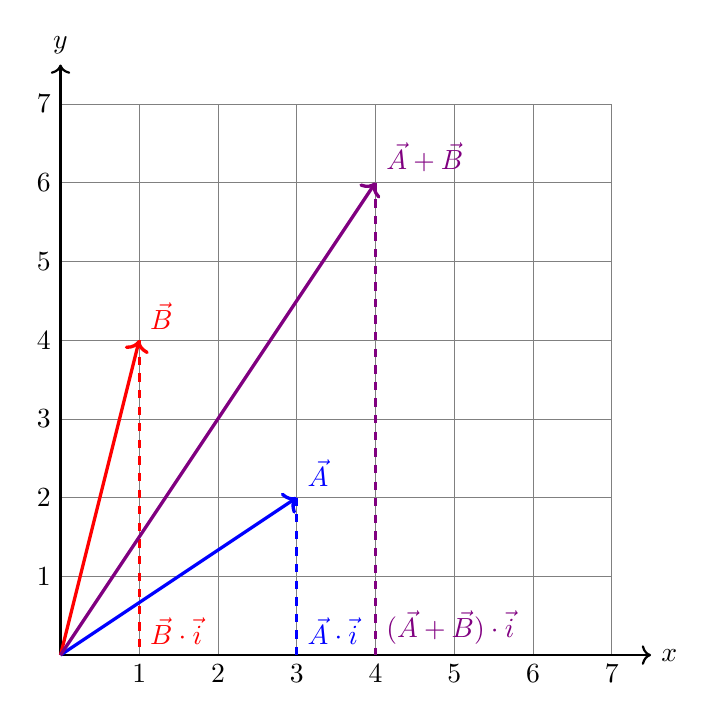
\begin{tikzpicture}
    % 1. Draw the grid with light gray, thin lines and 1cm step size
    \draw[step=1cm, gray, very thin] (0,0) grid (7,7);

    % 2. Draw the axes (optional, but helpful for context)
    \draw[->, thick] (0,0) -- (7.5,0) node[right] {$x$};
    \draw[->, thick] (0,0) -- (0,7.5) node[above] {$y$};

    % 3. Add coordinates for context (optional)
    \foreach \x in {1, 2, 3, 4, 5, 6, 7} {
        \node[below] at (\x, 0) {$\x$};
    }
    \foreach \y in {1, 2, 3, 4, 5, 6, 7} {
        \node[left] at (0, \y) {$\y$};
    }

    % 4. Draw a vector from the origin (0,0) to the point (3, 2)
    % The "->" option creates an arrow head
    \draw[->, very thick, blue] (0,0) -- (3,2) node[above right] {$\vec{A}$};

    % 4a. Draw a vector from the origin (0,0) to the point (3, 2)
    % The "->" option creates an arrow head
    \draw[dashed, very thick, blue] (3,2) -- (3,0) node[above right] {$\vec{A}\cdot\vec{i}$};
    
    % 5. Draw a vector from the origin (0,0) to the point (3, 2)
    % The "->" option creates an arrow head
    \draw[->, very thick, red] (0,0) -- (1,4) node[above right] {$\vec{B}$};
    
    % 5a. Draw a vector from the origin (0,0) to the point (3, 2)
    % The "->" option creates an arrow head
    \draw[dashed, very thick, red] (1,4) -- (1,0) node[above right] {$\vec{B}\cdot \vec{i}$};
    
    % 6. Draw a vector from the origin (0,0) to the point (3, 2)
    % The "->" option creates an arrow head
    \draw[->, very thick, violet] (0,0) -- (4,6) node[above right] {$\vec{A}+\vec{B}$};
    
    % 6. Draw a vector from the origin (0,0) to the point (3, 2)
    % The "->" option creates an arrow head
    \draw[dashed, very thick, violet] (4,6) -- (4,0) node[above right] {($\vec{A}+\vec{B})\cdot\vec{i}$};

\end{tikzpicture}
\end{center}
we can clearly see that $\vec{B}\cdot\vec{i} = 1$ and $\vec{A}\cdot\vec{i} = 3$ and $(\vec{A}+\vec{B})\cdot\vec{i} = 4$.\\

Now consider another simple expression $(\vec{A} +\vec{B})\cdot\vec{j}$\\
\begin{center}

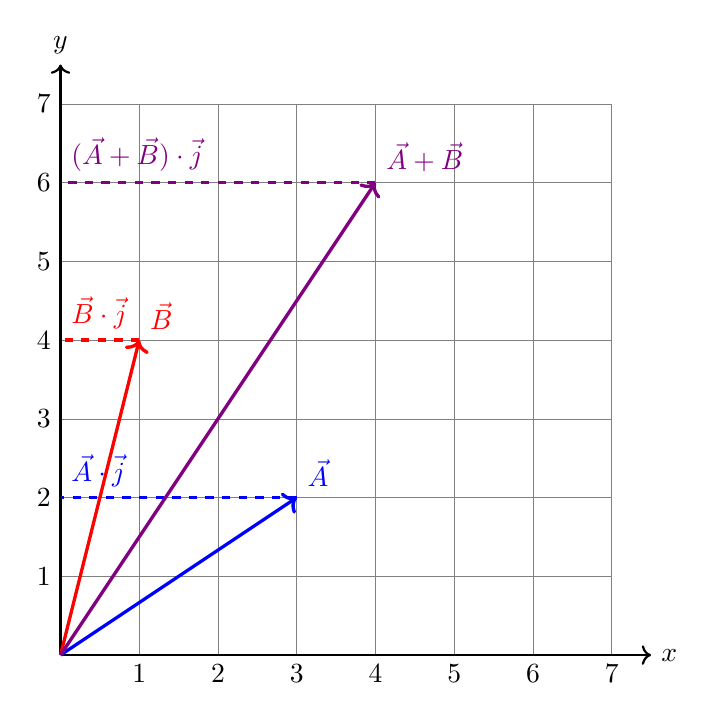
\begin{tikzpicture}
    % 1. Draw the grid with light gray, thin lines and 1cm step size
    \draw[step=1cm, gray, very thin] (0,0) grid (7,7);

    % 2. Draw the axes (optional, but helpful for context)
    \draw[->, thick] (0,0) -- (7.5,0) node[right] {$x$};
    \draw[->, thick] (0,0) -- (0,7.5) node[above] {$y$};

    % 3. Add coordinates for context (optional)
    \foreach \x in {1, 2, 3, 4, 5, 6, 7} {
        \node[below] at (\x, 0) {$\x$};
    }
    \foreach \y in {1, 2, 3, 4, 5, 6, 7} {
        \node[left] at (0, \y) {$\y$};
    }

    % 4. Draw a vector from the origin (0,0) to the point (3, 2)
    % The "->" option creates an arrow head
    \draw[->, very thick, blue] (0,0) -- (3,2) node[above right] {$\vec{A}$};

    % 4a. Draw a vector from the origin (0,0) to the point (3, 2)
    % The "->" option creates an arrow head
    \draw[dashed, very thick, blue] (3,2) -- (0,2) node[above right] {$\vec{A}\cdot\vec{j}$};
    
    % 5. Draw a vector from the origin (0,0) to the point (3, 2)
    % The "->" option creates an arrow head
    \draw[->, very thick, red] (0,0) -- (1,4) node[above right] {$\vec{B}$};
    
    % 5a. Draw a vector from the origin (0,0) to the point (3, 2)
    % The "->" option creates an arrow head
    \draw[dashed, very thick, red] (1,4) -- (0,4) node[above right] {$\vec{B}\cdot \vec{j}$};
    
    % 6. Draw a vector from the origin (0,0) to the point (3, 2)
    % The "->" option creates an arrow head
    \draw[->, very thick, violet] (0,0) -- (4,6) node[above right] {$\vec{A}+\vec{B}$};
    
    % 6. Draw a vector from the origin (0,0) to the point (3, 2)
    % The "->" option creates an arrow head
    \draw[dashed, very thick, violet] (4,6) -- (0,6) node[above right] {($\vec{A}+\vec{B})\cdot\vec{j}$};

\end{tikzpicture}
\end{center}
we can clearly see that $\vec{B}\cdot\vec{j} = 4$ and $\vec{A}\cdot\vec{j} = 2$ and $(\vec{A}+\vec{B})\cdot\vec{j} = 6$.\\

This allows for any inner product of the form $(\vec{a}+\vec{B})\cdot(\vec{i}+\vec{j})$.  For the general case of $\alpha \vec{i}+\beta\vec{j}$ it is easy to see that $\alpha$ and $\beta$ also distribute due to the Distribution Law of Algebra.

%section 2.6
\item Evalute $d F/dl$ for $F(P) = $ ``Distance from $P$ to point $A$" in a direction perpendicular to $AP$.

\BLUE{$F(P) = d(P, A)$.  Let $l$ be perpendicular to $AP$ at $P$.  For any $p \in l,\, F(P+p) \to F(P)$ as $p \to P$.  That is, $\partial F/\partial l = F(P)$.  Geometrically, consider a circle centered at $A$ and going through $P$.  The line $l \perp AP$ is a tangent line, thus $\partial F/\partial l$ is simply following along a circle of the same radius as $d(A,P)$.
}

\item Evaluate $dF/dl$ for $F(P) = $ ``1/(Distance from point $P$ to point $A$)" in the direction from $P$ to $A$.

\BLUE{$F(P) = 1/d(P,A)$.  Let $l$ be $AP$ and $p\in l$.  Then $F(P+p)=1/d(P-p,A)$ (minus as $p$ goes in the direction of $P$ to $A$.  The change with respect to $l$ is the derivative as $p \to P$ or 
\begin{align*}
	F'(P) &= \frac{d}{dP} \frac{1}{\sqrt{\SUM{i=1}3 (P_i-A_i)^2}} \\
		&= \PAREN{\frac{2\SUM{i=1}{3}P_i}{\sqrt{\SUM{i=1}3 (P_i-A_i)^2}}}^3
\end{align*}
}

\item Evaluate $dF/dl$ for $F(P) =$ ``Angle between $OA$ and $OP$", where $O$ and $A$ are two given points, in the direction from $P$ to $A$.

\item Evaluate $dF/dl$ for $F(P)=$ ``Distance from $P$ to the straight line that passes through $A$ and $B$", where $A$ and $B$ are given points in the direction parallel to $AB$.  The distance between a point $P$ and a staight line is defened as the shortest distance between $P$ and any of the points on the straight line.  The same definition applies to the distance between a point and a curve.

\item Evaluate $dF/dl$ for $F(P) = $ ``Area of a triangle $PAB$", where $A$ and $B$ are fixed points, in the direction parallel to $AB$.

\item Evaluate $dF/dl$ for $F(P)=$ ``Area of a triangle $PAB$", where $A$ and $B$ are fixed points, in the direction orhtogonal to $AB$.

%Section 2.7
\item Describe the gradient for each of the functions from the preceding exercises.

\item Give the geometric intuition behind equation (2.11). In other words, explain geometrically, why knowing the gradient is sufficient to determine the directional derivatives in all possible directions.

\BLUE{\begin{align*}
	\frac{dF}{dl} &= \nabla F\cdot \VK{L}
\end{align*}where $\VK{L}$ is the unit vector in the direction of $l$.  Interpreted directly, we can see that this means that change if $F$ in the $l$ is the projection of the gradient of $F$, $\nabla F$, onto the line $l$.  If, the $\nabla F$ is parallel to $l$ then $F$ has maximal changes along the line.  However, $\nabla F$ can be considered the normal vector to a plane.  This plan can be described by vectors perpendicular to each other and, by definition, perpendicular to $\nabla F$, thus forming a set of basis vectors.
}

%Section 2.8
\item Show that the length of $\VK{R}(\alpha+h)-\VK{R}(\alpha)$ is $2 \sin \frac{h}{2}$.

\item Confirm that the limit in (2.16) is 1 by L'Hopital's Rule.

\item Alternatively, recognize that the limit in (2.16) equals $\sin' 0 = \cos 0 = 1$.

\item Determine $\VK{R}''(\alpha)$.
\end{enumerate}

\end{document}